%%%%%%%%%% *** The Title %%%%%%%%%%
\title[]{기단\\\small{제8장}}

\begin{frame}[plain] %title page
	\titlepage
\end{frame}


\section{기단이란 무엇인가}



\begin{frame}[t]{기단이란?}
	\begin{tabular}{ll}
		\begin{minipage}[t]{0.45\textwidth}\scriptsize
			\begin{figure}[t]
				\includegraphics[trim=0 0 350 560, clip, page=249, width=\textwidth]{\bookfile}
			\end{figure}
		\end{minipage}	
		&
		\begin{minipage}[t]{0.5\textwidth} \scriptsize	
			\questionset{기단이란 무엇인가?}
			\solutionset{온도와 습도와 같은 물리적 특성이 유사한 공기 덩이
			수평 범위는 $1600\rm{~km}$ 이상, 두께는 수 $\rm{km}$ \newline}
			
			\questionset{기단의 발원지가 되기 위해 필요한 조건은 무엇인가?}
			\solutionset{1) 물리적으로 유사한 넓은 지역: \\
				ex) 해양 혹은 고도가 유사한 육지 \\
			2) 넓은 지역에서 대기 순환이 정체되어 대기가 지표면과 어느 정도 평형을 이룰 때까지 오랫동안 머물러야 함 \\
			ex) 무풍이나 풍속 약하고 정체하거나 느리게 움직이는 고기압 지역 \newline}
		
			\questionset{저기압 지역에서 기단이 잘 만들어질 수 없는 이유는 무엇인가?}
			\solutionset{공기가 수렴하므로 기온과 습도 속성과 별개로 다양한 성질의 대기를 그 구역으로 불러들임}
		
		\end{minipage}
	\end{tabular}
\end{frame}




\begin{frame}[t]{기단 기상}
	\begin{tabular}{ll}
		\begin{minipage}[t]{0.4\textwidth}\scriptsize
			\begin{figure}[t]
				\includegraphics[trim=330 290 50 135, clip, page=249, width=\textwidth]{\bookfile}
			\end{figure}
		\end{minipage}	
		&
		\begin{minipage}[t]{0.55\textwidth} \scriptsize	
			\questionset{기단 기상이란 무엇인가?}
			\solutionset{하나의 기단이 어떤 지역을 횡단하는데 며칠씩 걸릴 수 있는데, 기단의 영향을 받아 기상 조건이 일정한 상황을 기단 기상이라고 함. \newline}

			\questionset{캐나다 기단(오른쪽 그림)의 영향을 설명하라.}
			\solutionset{차고 건조한 캐나다 기단이 남쪽으로 이동하여 그 경로로에 있는 지역에 추운 날씨를 가져왔다. 그리고 기단 자신은 점점 따뜻해졌다.\newline}
			

			
		\end{minipage}
	\end{tabular}
\end{frame}


\section{기단의 분류}


\begin{frame}[t]{기단의 발원지}
	\begin{tabular}{ll}
		\begin{minipage}[t]{0.9\textwidth}\scriptsize
			\begin{figure}[t]
				\includegraphics[trim=50 30 50 480, clip, page=250, width=0.9\textwidth]{\bookfile}
			\end{figure}
		\end{minipage}	
	&
		\begin{minipage}[t]{0.05\textwidth}\scriptsize
			
		\end{minipage}	
	\end{tabular}
		
		\questionset{로키 산맥 동쪽의 미국 날씨에 가장 중요한 영향을 미치는 두 기단은 무엇인가?}
		\solutionset{로키 산맥 동쪽의 날씨에 큰 영향을 미치는 두 기단은 mT와 cP이다.
		cP 기단은 주로 겨울철에 한파를 몰아오고, mT 기단은 미국의 동쪽 2/3정도의 지역 강수의 주된 근원이다.}

\end{frame}


\begin{frame}[t]{기단의 분류}
	\begin{tabular}{ll}
		\begin{minipage}[t]{0.475\textwidth}\scriptsize

			\questionset{기단을 분류하는 기준은 무엇인가? 종류는?}
			\solutionset{\begin{figure}[t]
					\includegraphics[trim=50 450 350 260, clip, page=251, width=\textwidth]{\bookfile}
				\end{figure}
				발원지의 위도(기단 내의 기온 조건에 영향): 북극(A), 한대(P), 열대(T)\\
				기단과 접한 지표면의 상태(기단 내의 습도 조건에 영향): 대륙(c), 해양(m)\\
				cA: 대륙성 북극기단(매우 차갑고 건조) \\
				cP: 대륙성 한대기단(차갑고 건조) \\
				cT: 대륙성 열대기단(따뜻하고 건조) \\
				mT: 해양성 열대기단(따뜻하고 습함) \\
				mP: 해양성 한대기단(차갑고 습함)}
		\end{minipage}	
		&
		\begin{minipage}[t]{0.475\textwidth}\scriptsize
			\questionset{mA가 없는 까닭은?}
			\solutionset{북극기단이 북극 해양 위에서 형성된다고 하더라도, 이 바다는 1년 내내 얼음으로 뒤덮여 있어 여기서 발원한 기단은 대륙에서 형성된 기단과 연속적인 습도 특성을 갖게 된다.\newline}
			
			\questionset{기단과 관련하여 소문자 k와 w가 의미하는 것은 무엇이며, 이를 기단의 안정성과 관련하여 논의하시오.}
			\solutionset{만약 기단이 이동해가는 표면보다 더 춥다면 k, 지표면보다 더 덥다면 w를 쓴다. 즉, k나 w는 기단 자체의 따뜻하고 차가운 것을 나타낸 것이 아니라 기단이 지나가는 지역의 지표면에 비해 상대적인 차이를 나타낸다. 
			k 기단은 아래로부터 가열되어 보다 불안정해져 적운형 구름이 형성되고, 혹시 비가 내린다면 천둥을 동반할 수 있다. w 기단은 아래로부터 냉각되어 보다 안정해져 층운형 구름이 형성되고, 혹시 비가 내린다면 가벼운 비가 내릴 것이다. }
			
		\end{minipage}	
	\end{tabular}
	
	
\end{frame}





\begin{frame}[t]{우리나라에 영향을 미치는 기단}
	\begin{tabular}{ll}
		\begin{minipage}[t]{0.35\textwidth}\scriptsize
			\begin{figure}[t]
				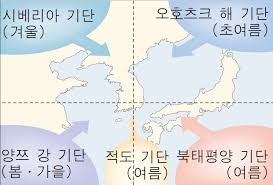
\includegraphics[width=\textwidth]{./images/AirMass1}
			\end{figure}
		\end{minipage}	
		&
		\begin{minipage}[t]{0.6\textwidth} \scriptsize	
		\questionset{우리나라 날씨에 중요한 영향을 미치는 기단은 무엇인가?}
		\solutionset{\begin{table}[h]
				\resizebox{\textwidth}{!}{%
					\begin{tabular}{c|c|c|c}
						\hline
						기단        & 성질    & 시기            & 영향                 \\ \hline
						시베리아 기단   & 한랭 건조 & 주로 겨울         & 삼한 사온 현상, 혹한, 꽃샘추위 \\ \hline
						양쯔 강 기단   & 온난 건조 & 봄, 가을         & 따뜻하고 건조한 날씨        \\ \hline
						북태평양 기단   & 고온 다습 & 주로 여름         & 적란운과 소나기, 열대야 현상   \\ \hline
						오호츠크 해 기단 & 한랭 다습 & 초여름 $\sim$장마철 & 동해안의 냉량, 높새바람      \\ \hline
						적도 기단     & 고온 다습 & 여름            & 태풍                 \\ \hline
					\end{tabular}%
				}
			\end{table}}
			
		\end{minipage}
	\end{tabular}
\end{frame}








\section{기단의 변질}



\begin{frame}[t]{기단의 변질}
	\begin{tabular}{ll}
		\begin{minipage}[t]{0.5\textwidth}\scriptsize
			\begin{figure}[t]
				\includegraphics[trim=50 340 240 50, clip, page=252, width=\textwidth]{\bookfile}
			\end{figure}
		\end{minipage}	
		&
		\begin{minipage}[t]{0.45\textwidth} \scriptsize	
			\questionset{오른쪽 그림의 cP 기단이 바다 위를 지나갈 때 나타나는 변화를 설명하시오.}
			\solutionset{cP 기단이 대서양으로 이동하면, 수면으로부터 증발된 다량의 수증기가 기단으로 빠르게 이동하고, 지표면의 따뜻한 물이 대기 하부를 가열하여 기단을 불안정하게 만들고 상승기류를 발달시킨다. \\
			결국 대륙의 대기가 불안정한 mP기단으로 변화한다.}
			
		\end{minipage}
	\end{tabular}
\end{frame}




\section{북미 기단의 성격}



\begin{frame}[t]{북미 기단의 성질}
	\begin{tabular}{ll}
		\begin{minipage}[t]{0.7\textwidth}\scriptsize
			\begin{figure}[t]
				\includegraphics[trim=30 350 50 50, clip, page=253, width=\textwidth]{\bookfile}
			\end{figure}
		\end{minipage}	
		&
		\begin{minipage}[t]{0.05\textwidth} \scriptsize	
			
			
		\end{minipage}
	\end{tabular}
\end{frame}




\begin{frame}[t]{대륙성 한대기단(cP)과 대륙성 북극기단(cA)}
	\begin{tabular}{ll}
		\begin{minipage}[t]{0.45\textwidth}\scriptsize
			\begin{figure}[t]
				\includegraphics[trim=50 420 320 50, clip, page=254, width=\textwidth]{\bookfile}
			\end{figure}
		\end{minipage}	
		&
		\begin{minipage}[t]{0.5\textwidth} \scriptsize	

			\questionset{대륙성 북극 기단의 냉각효과를 설명하시오.}
			\solutionset{대륙성 북극 기단은 한랭 건조하다. 미국의 중부와 동부 지역 대부분에 나타나는 겨울철 한파는 북극 기단의 팽창과 관련이 있다. 북극 제트기류로 미국 중부와 동부가 북극 기단으로 덮이게 되면 극한의 추위가 나타나게 된다. \newline}
			
		
			
		\end{minipage}
	\end{tabular}
\end{frame}



\begin{frame}[t]{시베리아 특급}
	\begin{tabular}{ll}
		\begin{minipage}[t]{0.5\textwidth}\scriptsize
			\begin{figure}[t]
				\includegraphics[trim=255 350 50 110, clip, page=255, width=\textwidth]{\bookfile}
			\end{figure}
		\end{minipage}	
		&
		\begin{minipage}[t]{0.45\textwidth} \scriptsize	
			\questionset{시베리아 특급 이란 무엇인가?}
			\solutionset{겨울철 대륙위에 형성된 거대한 고기압은 북극권 근처의 넓은 빙결지역에서 형성된 찬 cP 기단이 남하하여 한파를 몰고 오는 현상이다.}
			
		\end{minipage}
	\end{tabular}
\end{frame}





\begin{frame}[t]{호수 효과 눈(lake-effect snow)}
	\begin{tabular}{ll}
		\begin{minipage}[t]{0.45\textwidth}\scriptsize
			\begin{figure}[t]
				\includegraphics[trim=30 30 320 480, clip, page=257, width=\textwidth]{\bookfile}
			\end{figure}
		\end{minipage}	
		&
		\begin{minipage}[t]{0.5\textwidth} \scriptsize	
			\begin{figure}[t]
				\includegraphics[trim=350 450 50 50, clip, page=257, width=0\textwidth]{\bookfile}
			\end{figure}
			\questionset{cP 기단이 겨울철 오대호를 가로 질러 이동함에 따라 발생하는 호수 효과 눈(lake-effect snow)을 설명하라.}
			\solutionset{캐나다 중부지방에서 발원한 cP기단은 차갑고 안정하다. 가을철이나 초겨울에 기단이 오대호를 지나면서 cPk 기단으로 변질된다. 따뜻한 호수 표면으로부터 공급된 열과 수증기는 기단을 불안정하게 만들고, 호수를 지나 지상으로 올라와 냉각되고 많은 양의 호수 효과 눈(lake-effect snow)을 내리게 한다.\newline}
			
			%			\questionset{호수 효과에 의한 눈보라를 설명하시오.}
			%			\solutionset{오하이오 호 북동부는 이리 호의 강설대에 속한다. 차아운 기단이 비교적 따뜻한 이리 호를 지나면서 가열되고, 수증기가 공급되어 호수 효과 강우와 스콜성 강우와 스콜성 눈을 내리게 한다. }
			
		\end{minipage}
	\end{tabular}
\end{frame}




\begin{frame}[t]{호수 효과에 의한 강설량 차이}
	\begin{tabular}{ll}
		\begin{minipage}[t]{0.5\textwidth}\scriptsize
			\begin{figure}[t]
				\includegraphics[trim=50 30 165 520, clip, page=254, width=\textwidth]{\bookfile}\\
				\includegraphics[trim=50 550 320 80, clip, page=256, width=0.8\textwidth]{\bookfile}
			\end{figure}
		\end{minipage}	
		&
		\begin{minipage}[t]{0.45\textwidth} \scriptsize	
			
			\questionset{썬더 베이와 마켓의 월별 강설량 차이가 나타나는 이유는 무엇인가?\\
				\begin{figure}[t]
					\includegraphics[trim=20 30 345 630, clip, page=255, width=0.8\textwidth]{\bookfile}
			\end{figure}}
			\solutionset{오대호 호수의 물은 여름철에 태양으로부터 에너지를 흡수했다가, 찬 cP 기단이 호수를 지나면서 변질되는 호수 효과 눈(lake-effect snow)으로 설명할 수 있다. }
			
		\end{minipage}
	\end{tabular}
\end{frame}






\begin{frame}[t]{해양성 한대기단(mP)}
	\begin{tabular}{ll}
		\begin{minipage}[t]{0.45\textwidth}\scriptsize
			\begin{figure}[t]
				\includegraphics[trim=350 50 30 550, clip, page=256, width=\textwidth]{\bookfile}
			\end{figure}
			\questionset{태평양의 mP기단은 어떻게 생성되는 지 설명하시오.}
			\solutionset{태평양의 mP기단은 시베리아의 cP기단으로부터 시작된다. 시베리아의 cP기단이 동쪽으로 움직이면서 따뜻한 해양으로부터 수증기를 얻고, 북아메리카의 서쪽 해안에 도달하게 되는데 자주 낮은 구름과 비를 동반한다. \newline}

		\end{minipage}	
		&
		\begin{minipage}[t]{0.5\textwidth} \scriptsize	
			\questionset{겨울철 한대 기단은 한랭하다. 겨울철에 mP와 cP 기단 중 어느 기단이 더 한랭한지 추정하고 그 이유를 설명하시오.}
			\solutionset{대륙성 극 기단은 해양성 극 기단보다 공기가 건조하기 때문에 차갑다. 해양성 극 기단에 존재하는 수증기는 온도 효과를 완화시켜주는 역할을 한다. 같은 이유로 대륙성 열대 기단은 해양성 열대 기단보다 건조하기 때문에 더 덥다. \newline}
			
			\questionset{어떤 기단이 태평양 해안의 기상에 가장 큰 영향을 미치는가?}
			\solutionset{북태평양의 mP기단은 우리가 살고 있는 태평양 해안 지역의 날씨에 중요하다. 북태평양 mT기단은 북아메리카의 날씨에 많은 영향을 주지는 않는다.\\
			기단이 북쪽 방향으로 이동하면, 하층이 냉각되어 보다 안정하게 되고 안개나 이슬비가 내리거나 일상적인 강수가 내리게 된다.}
			
		\end{minipage}
	\end{tabular}
\end{frame}



\begin{frame}[t]{북대서양의 해양성 한대기단}
	\begin{tabular}{ll}
		\begin{minipage}[t]{0.5\textwidth}\scriptsize
			\begin{figure}[t]
				\includegraphics[trim=285 30 50 450, clip, page=258, width=\textwidth]{\bookfile}
			\end{figure}
		\end{minipage}	
		&
		\begin{minipage}[t]{0.45\textwidth} \scriptsize	
			\questionset{북대서양의 mP기단과 연관된 노이스터(nor’easter)를 설명하시오.}
			\solutionset{대서양의 mP기단의 침입과 관련된 기상을 국지적으로 노이스터라고 한다. 강한 북동풍, 빙점에 가까운 기온, 높은 상대습도, 강우 가능성으로 인해 환영 받지 못하는 기상 현상이다. }
			
		\end{minipage}
	\end{tabular}
\end{frame}



\begin{frame}[t]{해양성 열대기단(mT)}
	\begin{tabular}{ll}
		\begin{minipage}[t]{0.45\textwidth}\scriptsize
			\begin{figure}[t]
				\includegraphics[trim=0 430 220 0, clip, page=260, width=\textwidth]{\bookfile}
			\end{figure}
		\end{minipage}	
		&
		\begin{minipage}[t]{0.5\textwidth} \scriptsize	
			\questionset{미국 동부와 중부에 가장 많은 양의 습기를 제공하는 기단과 그 발원지는 어디인가?}
			\solutionset{멕시코 만, 캐러비안 해, 대서양의 mT 기단이다. 이 mT기단은 낮 동안 대륙으로 이동하면서 mTk로 변질되며 불안정성이 증가한다. }
		\end{minipage}
	\end{tabular}
\end{frame}



\begin{frame}[t]{대기의 강(atmospheric river)}
	\begin{tabular}{ll}
		\begin{minipage}[t]{0.55\textwidth}\scriptsize
			\begin{figure}[t]
				\includegraphics[trim=30 460 290 50, clip, page=261, width=\textwidth]{\bookfile}
			\end{figure}
		\end{minipage}	
		&
		\begin{minipage}[t]{0.4\textwidth} \scriptsize	
			\questionset{Pineapple Express가 무엇인지 설명하시오.}
			\solutionset{북태평양의 아열대 해상에서 발원하는 mT기단은 하와이섬에 근접한 해수로부터 남캘리포니아나 다른 서쪽 해안 지역으로 특별히 강한 강수현상을 일으킬 수 있는 수증기의 강한 흐름을 만들어내는데 이를 Pineapple Express라고 한다.}
			
		\end{minipage}
	\end{tabular}
\end{frame}



\begin{frame}[t]{Pineapple Express의 생성 과정}
	\begin{tabular}{ll}
		\begin{minipage}[t]{0.5\textwidth}\scriptsize
			\begin{figure}[t]
				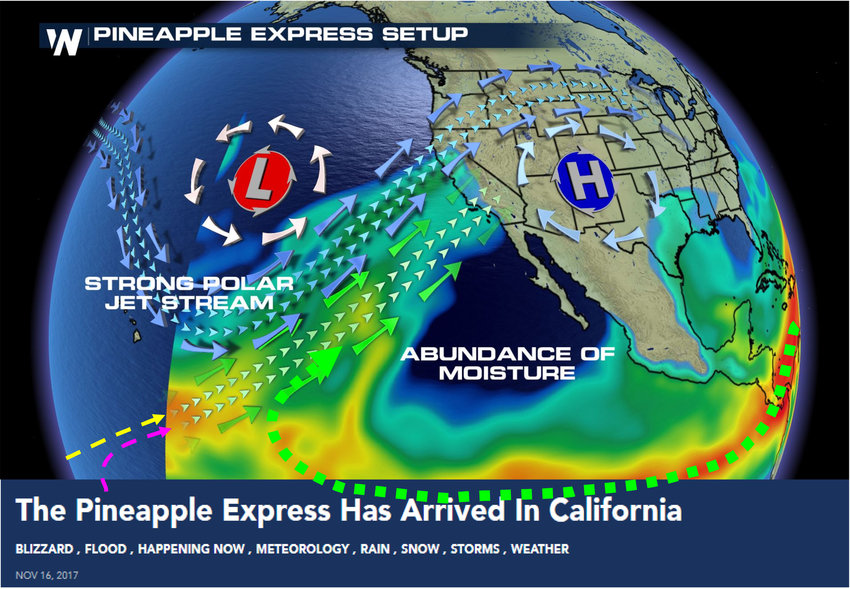
\includegraphics[width=\textwidth]{./images/pineapple_express}
			\end{figure}
		\end{minipage}	
		&
		\begin{minipage}[t]{0.45\textwidth} \scriptsize	
			알래스카의 걸프만을 통과하는 겨울 폭풍의 침강 결과이다. 이 폭풍은 다습하고 선선한 mP 기단에 의해 나타난다. \\
			그러나 수년 동안, 강한 남부 한대 제트는 북동 하와이로부터 서해안에 이르는 열대에서 수증기와 따뜻한 mT 대기를 수송하는 통로 역할을 하였다. 이 mT 기단은 시에라네바다 지역의 낮은 지역에 폭설과 집중 호우를 가져올 수 있는 폭풍 시스템을 만든다. 
			
		\end{minipage}
	\end{tabular}
\end{frame}


\begin{frame}[t]{해양성 열대기단과 강수량}
	\begin{tabular}{ll}
		\begin{minipage}[t]{0.45\textwidth}\scriptsize
			\begin{figure}[t]
				\includegraphics[trim=50 50 320 500, clip, page=260, width=\textwidth]{\bookfile}
			\end{figure}
		\end{minipage}	
		&
		\begin{minipage}[t]{0.5\textwidth} \scriptsize	
		\questionset{미국 동부지역의 연평균 강수량은 어떤 변화를 보이는가?}
		\solutionset{mT 기단의 발원지인 멕시코만으로부터 거리가 멀어짐에 따라 연 강수량이 전체적으로 감소한다. }
			
		\end{minipage}
	\end{tabular}
\end{frame}



%\begin{frame}[t]{대륙성 열대기단}
%	\begin{tabular}{ll}
%		\begin{minipage}[t]{0.65\textwidth}\scriptsize
%			\begin{figure}[t]
%				\includegraphics[trim=50 290 50 50, clip, page=218, width=\textwidth]{\bookfile}
%			\end{figure}
%		\end{minipage}	
%		&
%		\begin{minipage}[t]{0.3\textwidth} \scriptsize	
%			\questionset{미국 동부지역의 연평균 강수량은 어떤 변화를 보이는가?}
%			\solutionset{mT 기단의 발원지인 멕시코만으로부터 거리가 멀어짐에 따라 연 강수량이 전체적으로 감소한다. }
%			
%		\end{minipage}
%	\end{tabular}
%\end{frame}
%
